\subsection{第 20 课 | 字符串算法}

\subsubsection{脑图}

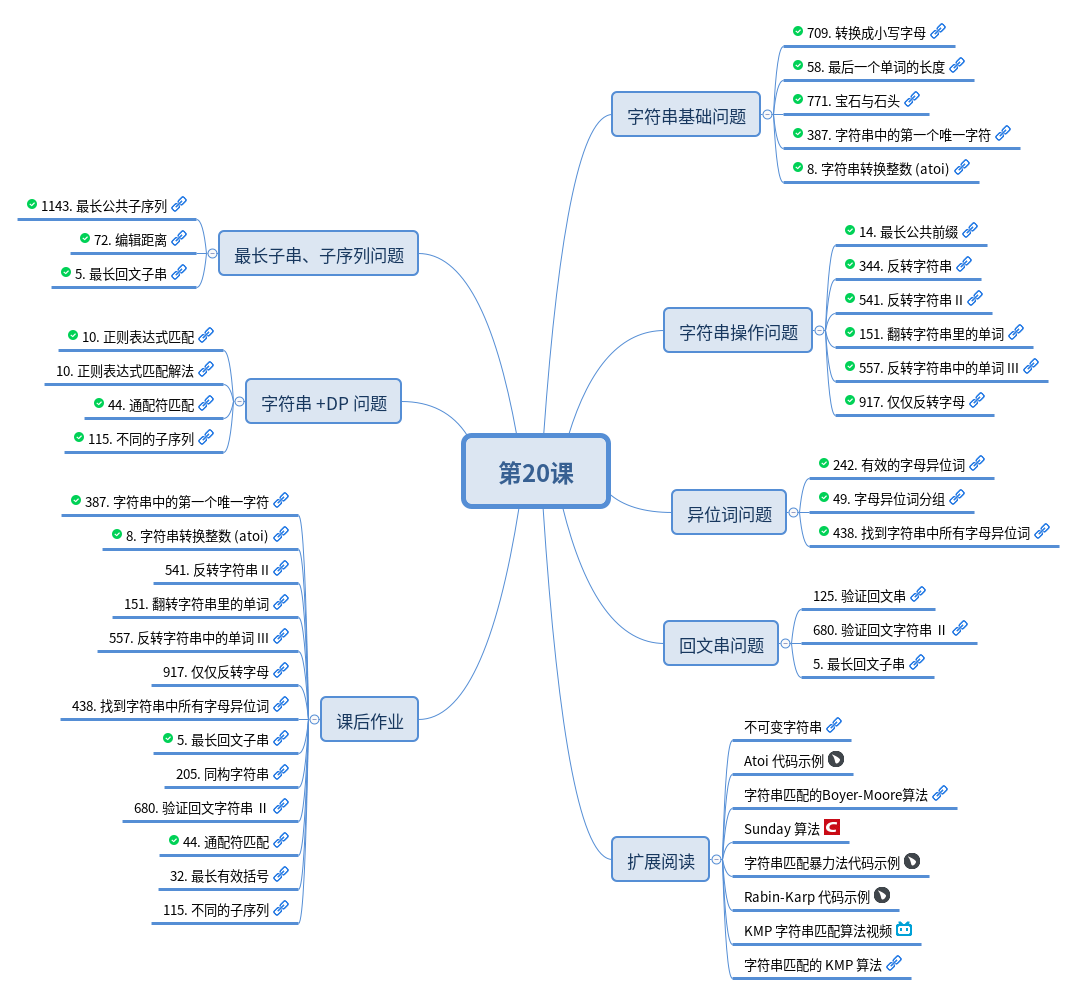
\includegraphics[width=150mm,height=140mm]{images/camp/第20课.png}

\subsubsection{题目}

\paragraph{字符串基础问题}

\begin{itemize}
  \item \hyperref[leetcode:709]{709. 转换成小写字母}
  \item \hyperref[leetcode:58]{58. 最后一个单词的长度}
  \item \hyperref[leetcode:771]{771. 宝石与石头}
  \item \hyperref[leetcode:387]{387. 字符串中的第一个唯一字符}
  \item \hyperref[leetcode:8]{8. 字符串转换整数 (atoi)}
\end{itemize}

\paragraph{字符串操作问题}

\begin{itemize}
  \item \hyperref[leetcode:14]{14. 最长公共前缀}
  \item \hyperref[leetcode:344]{344. 反转字符串}
  \item \hyperref[leetcode:541]{541. 反转字符串 II}
  \item \hyperref[leetcode:151]{151. 翻转字符串里的单词}
  \item \hyperref[leetcode:557]{557. 反转字符串中的单词 III}
  \item \hyperref[leetcode:917]{917. 仅仅反转字母}
\end{itemize}

\paragraph{异位词问题}

\begin{itemize}
  \item \hyperref[leetcode:242]{242. 有效的字母异位词}
  \item \hyperref[leetcode:49]{49. 字母异位词分组}
  \item \hyperref[leetcode:438]{438. 找到字符串中所有字母异位词}
\end{itemize}

\paragraph{回文串问题}

\begin{itemize}
  \item \hyperref[leetcode:125]{125. 验证回文串}
  \item \hyperref[leetcode:680]{680. 验证回文字符串 Ⅱ}
  \item \hyperref[leetcode:5]{5. 最长回文子串}
\end{itemize}

\paragraph{最长子串、子序列问题}

\begin{itemize}
  \item \hyperref[leetcode:1143]{1143. 最长公共子序列}
  \item \hyperref[leetcode:72]{72. 编辑距离}
  \item \hyperref[leetcode:5]{5. 最长回文子串}
\end{itemize}

\paragraph{字符串 + DP 问题}

\begin{itemize}
  \item \hyperref[leetcode:10]{10. 正则表达式匹配}
  \item \hyperref[leetcode:44]{44. 通配符匹配}
  \item \hyperref[leetcode:115]{115. 不同的子序列}
\end{itemize}

\paragraph{课后作业}

\begin{itemize}
  \item \hyperref[leetcode:387]{387. 字符串中的第一个唯一字符}
  \item \hyperref[leetcode:8]{8. 字符串转换整数 (atoi)}
  \item \hyperref[leetcode:541]{541. 反转字符串 II}
  \item \hyperref[leetcode:151]{151. 翻转字符串里的单词}
  \item \hyperref[leetcode:557]{557. 反转字符串中的单词 III}
  \item \hyperref[leetcode:917]{917. 仅仅反转字母}
  \item \hyperref[leetcode:438]{438. 找到字符串中所有字母异位词}
  \item \hyperref[leetcode:5]{5. 最长回文子串}
  \item \hyperref[leetcode:205]{205. 同构字符串}
  \item \hyperref[leetcode:680]{680. 验证回文字符串 Ⅱ}
  \item \hyperref[leetcode:44]{44. 通配符匹配}
  \item \hyperref[leetcode:32]{32. 最长有效括号}
  \item \hyperref[leetcode:115]{115. 不同的子序列}
\end{itemize}

\subsubsection{扩展阅读}

\href{https://www.ruanyifeng.com/blog/2013/05/boyer-moore_string_search_algorithm.html}{Boyer-Moore 算法} \\
\href{https://blog.csdn.net/u012505432/article/details/52210975}{Sunday 算法} \\
\href{https://www.bilibili.com/video/av11866460?from=search&seid=17425875345653862171}{KMP 字符串匹配算法视频} \\
\href{http://www.ruanyifeng.com/blog/2013/05/Knuth%E2%80%93Morris%E2%80%93Pratt_algorithm.html}{字符串匹配的 KMP 算法}
